% Condensed conference version (target: ~6 pages, IEEEtran conference class).
% Every number is taken from kgxai_paper.tex (the full version); nothing new is claimed here.
\documentclass[conference]{IEEEtran}
\IEEEoverridecommandlockouts

\usepackage{cite}
\usepackage{amsmath,amssymb,amsfonts}
\usepackage{graphicx}
\usepackage{textcomp}
\usepackage{xcolor}
\usepackage{booktabs}
\usepackage{url}
\usepackage[hidelinks]{hyperref}

\begin{document}

\title{Knowledge-Graph-Guided Consistency Checking for\\ Stroke Infarct Segmentation from CT Imaging}

\author{
\IEEEauthorblockN{Ekanath D V}
\IEEEauthorblockA{\textit{School of Computer Science and Engineering} \\
\textit{Vellore Institute of Technology}\\
Chennai, India \\
23MIA1023}
\and
\IEEEauthorblockN{Rohan Julius Preetan}
\IEEEauthorblockA{\textit{School of Computer Science and Engineering} \\
\textit{Vellore Institute of Technology}\\
Chennai, India \\
23MIA1160}
}

\maketitle

\begin{abstract}
Deep models for acute ischemic stroke triage often produce outputs that are never checked against each other or against vascular anatomy, so a model can place an infarct on the side opposite the detected occlusion. We build KG-XAI, which encodes a patient-specific Circle-of-Willis (CoW) vessel graph and a guideline rule graph, injects the vessel graph into a SegResNet decoder through a graph attention network (GAT) and zero-initialized cross-attention, and adds a differentiable laterality-consistency loss. Before using any guideline rule as a constraint, we test it on the public ISLES'24 cohort: of seven candidate rules, only laterality is supported (94.7\% agreement, $n=94$). We then evaluate on a pre-registered 3-fold $\times$ 3-seed grid. Mean strict Joint-Decision Consistency Rate (JDCR) is higher for the graph model (0.965 vs.\ 0.749), but this is driven by two collapsed baseline runs; when both train normally, Dice ($p=0.59$, $n=148$) and JDCR ($p=0.84$) do not differ. A random same-size graph and a forced-open attention gate also leave Dice unchanged, so the learned graph pathway does not improve accuracy. The graph is useful in a non-learned role: a ground-truth-free check built from it (wrong-side or sub-1\,mL prediction) detects severe segmentation failure with AUROC 0.836, against 0.583 for ensemble disagreement, and its unique catches contain no false positives. MC-dropout is competitive on subtler failures. We report all results, including negative ones.
\end{abstract}

\begin{IEEEkeywords}
stroke, knowledge graph, graph attention network, medical image segmentation, failure detection, explainable AI
\end{IEEEkeywords}

\section{Introduction}
Endovascular thrombectomy decisions for large-vessel-occlusion (LVO) stroke depend on the occlusion, collateral circulation and infarct extent. Multi-task CT systems predict these with separately supervised heads \cite{luan2026}, so nothing in training checks that the outputs are mutually consistent. A clinician reviewing such output cannot tell whether the numbers hang together.

We ask whether encoding vascular anatomy and guideline knowledge as a graph (a) improves segmentation and (b) makes predictions more trustworthy. We use the public ISLES'24 data \cite{isles2024}. The base paper's training data and 7-center split are not public, so we reimplement the setting and compare three models we train ourselves on identical data, splits and seeds: \textbf{B0}, a SegResNet baseline with no graph; \textbf{B1}, B0 plus GAT-based graph injection; and \textbf{B2}, B1 plus a laterality-consistency loss.

Contributions:
\begin{enumerate}
\item A two-layer knowledge graph: a 12-node CoW vessel graph built from each patient's own vessel mask, and a guideline graph (16 concepts, 7 rules) with sources checked against primary records.
\item A validate-before-constrain protocol: each guideline rule is tested against ground truth before use. Only 1 of 7 survives.
\item A zero-initialized graph-injection architecture and a laterality-consistency loss, with the Joint-Decision Consistency Rate (JDCR) and a deterministic, LLM-free rationale.
\item A pre-registered 3-fold $\times$ 3-seed evaluation, plus mechanism-level ablations, showing the learned graph pathway does not improve accuracy.
\item A ground-truth-free, graph-based failure detector, benchmarked against ensemble disagreement and MC-dropout.
\end{enumerate}

\section{Related Work}
Stroke imaging work mostly treats LVO detection, collateral scoring and infarct segmentation separately; ISLES \cite{isles2024} drives public infarct-segmentation benchmarking, and \cite{luan2026} trains all three jointly but scores them independently. GNNs and knowledge graphs have been used to inject structured priors into imaging models. Our vessel graph is patient-specific (coordinates and vessel presence come from that patient's mask, not an atlas), and our guideline rules are tested before use. Constraint-based training has precedent in logic-constrained learning; we constrain only on the one rule verified in the cohort. For uncertainty, we compare against deep ensembles \cite{lakshminarayanan2017} and MC-dropout \cite{gal2016dropout}.

\section{Data}
ISLES'24 provides 149 subjects from 2 centers (148 usable). Each has admission NCCT, CTA, CBF, CBV, MTT and Tmax maps, a CoW vessel mask, an admission occlusion mask, and a follow-up diffusion-weighted infarct mask, resampled to 1\,mm isotropic space. Four properties of this release limit what is learnable:
\begin{itemize}
\item No timing data (empty for 149/149), so time-window criteria are not evaluable.
\item No ASPECTS or collateral grade; we use the hypoperfusion intensity ratio (HIR) \cite{olivot2014} as a proxy.
\item Only 4 of 149 subjects are LVO-negative, so binary LVO detection is not viable.
\item The target is the \emph{final} (follow-up) infarct, which also depends on treatment response.
\end{itemize}
All model inputs come from admission data only; the follow-up mask is used only as the training target and for rule validation.

\section{Method}
\subsection{Pipeline}
A shared SegResNet \cite{myronenko2018} segments the follow-up infarct from a lesion-centered $128{\times}128{\times}64$ patch of the 6-channel admission volume. The same encoder also processes a whole-brain view, so the CoW is always in frame. Twelve per-patient vessel coordinates are trilinearly sampled from its stage-1 features and passed through a 2-layer GAT \cite{velickovic2018} (2 heads, hidden size 32) over the fixed CoW edges. The 12 vessel embeddings are injected into every decoder stage by cross-attention. A rule evaluator then scores each prediction and writes a template rationale (Fig.~\ref{fig:arch}).


% --- Architecture figure: save your diagram as figures/fig_architecture.png ---
\begin{figure*}[t]
\centering
\IfFileExists{figures/fig_architecture.png}{\includegraphics[width=0.9\textwidth]{figures/fig_architecture.png}}{%
\fbox{\parbox[c][5.5cm][c]{0.85\textwidth}{\centering\large [Placeholder -- architecture diagram:\\ place \texttt{figures/fig\_architecture.png}]}}}
\caption{KG-XAI architecture. A shared SegResNet encodes a lesion-centered patch and a whole-brain view; vessel coordinates sampled from the whole-brain features feed a 2-layer GAT, whose 12 node embeddings are injected into every decoder stage by zero-initialized cross-attention. A rule evaluator scores each predicted mask.}
\label{fig:arch}
\end{figure*}

\subsection{Knowledge graph}
\textbf{Layer 1 (vessel graph).} Twelve nodes and 12 edges (ICA, MCA, ACA, PCA, Acom, Pcom, BA), with topology from TopCoW \cite{topcow2023} and published adjacency \cite{alastruey2007}. Anatomical variants are \emph{absent nodes} (a per-patient presence flag), not different edges. A vessel is marked occluded only if the occlusion-mask centroid lies within 15\,mm of its node; without this gate the basilar node falsely matches 19 of 20 low-confidence cases.

\textbf{Layer 2 (guideline graph).} Sixteen concepts and seven plausibility rules drawn from DAWN \cite{dawn2018}, DEFUSE-3 \cite{defuse3_2018}, the AHA/ASA guideline \cite{ahaasa2026} and HIR studies \cite{olivot2014}.

\subsection{Zero-initialized cross-attention}
At each decoder stage, spatial features form query tokens attended against the 12 vessel embeddings (4 heads; absent nodes masked). The output is added back through a learned scalar gate $g$ initialized to zero:
\begin{equation}
x' = x + g\cdot \mathrm{Attn}(Q,K,V), \qquad g \leftarrow 0 \text{ at init.}
\end{equation}
At epoch 0 the model is therefore identical to the plain trunk (maximum output difference 0.0 on the validation set), so the graph can only help through training.

\subsection{Laterality-consistency loss and JDCR}
Let $p_{\text{fg}}(v)$ be the predicted foreground probability at whole-brain voxel $v$ and $s$ the expected infarct side, taken from the admission occlusion only. The loss is the share of predicted mass on the wrong side of the per-subject midline:
\begin{equation}
\mathcal{L}_{\text{lat}}=\frac{\sum_{v:\,\mathrm{side}(v)\neq s}p_{\text{fg}}(v)}{\sum_v p_{\text{fg}}(v)+\varepsilon},\quad
\mathcal{L}=\mathcal{L}_{\text{seg}}+\lambda\mathcal{L}_{\text{lat}},
\end{equation}
with $\lambda=0.1$. The weight is small because 5.3\% of ground-truth cases violate strict laterality.

At evaluation, a subject is \emph{consistent} if under 50\% of the predicted lesion lies on the wrong side, and \emph{evaluable} if it has a known side and a non-empty prediction. JDCR is the share of evaluable subjects that are consistent. We report \emph{strict} JDCR, where an empty prediction counts against the model, so a model cannot raise JDCR by abstaining. Rationales are filled-in templates built from the same computed values, with no language model.

\section{Rule Validation}
Each rule was tested against the follow-up infarct with the pass mark fixed beforehand (Table~\ref{tab:rules}). Only laterality holds. The two most decisive rejected tests also fail independently in both acquisition centers. A likely cause is that every subject in this release was successfully reperfused, so admission-time rules need not predict final infarct size. We do not claim the rules are wrong in general, only that they do not hold in this cohort.

\begin{table}[t]
\centering
\caption{Plausibility-rule validation on ISLES'24.}
\label{tab:rules}
\footnotesize
\begin{tabular}{p{3.6cm}p{3.3cm}c}
\toprule
\textbf{Rule} & \textbf{Result} & \textbf{Status} \\
\midrule
Infarct on occluded side & 89/94 = 94.7\% & Supported \\
Proximal occlusion $\Rightarrow$ larger infarct & medians 13.8 vs.\ 13.1\,mL, $p=0.66$ & Rejected \\
Good collaterals limit infarct (HIR) & $\rho=0.05$, $p=0.54$ & Rejected \\
Poor collaterals $\Rightarrow$ larger infarct & $p=0.13$ & Rejected \\
HIR behaves as collateral signal & $\rho=+0.19$ (wrong sign) & Rejected \\
Infarct within Tmax\,$>$6\,s region & median 0.51 (mark 0.70) & Rejected \\
Large infarct needs occlusion & only 4 negatives & Untestable \\
\bottomrule
\end{tabular}
\end{table}

\section{Experiments}
\subsection{Setup}
All models use 100 epochs, MONAI augmentation, the same 6-channel input, and a warm start from the same pretrained SegResNet trunk. B0 and B2 are trained on 3 folds $\times$ 3 seeds (9 runs each); B1 on fold 0 $\times$ 3 seeds. Pass marks were fixed before the runs. The primary claim is that B2's mean strict JDCR exceeds B0's. The guard rail is that B2's mean Dice is at most 0.02 below B0's. Segmentation is scored with the official ISLES'24 metrics.

\subsection{Measurement checks}
Two bugs were found and fixed before drawing conclusions. First, an early JDCR scored all models on a downscaled view that only B2 had been trained to segment, which made B0 and B1 look like they abstained on half the subjects; all models are now scored on their full-resolution predictions. Second, the B0 JDCR we first cited came from a shelved multi-task checkpoint, not B0; the loader was fixed and all 21 checkpoints re-scored.

\subsection{Auxiliary heads (negative result)}
LVO-localization and collateral heads were tried in four regimes (pooled features, per-vessel GNN, GNN with augmentation, GNN with frozen encoder). All fall below the majority-class baseline (LVO 52--56\% vs.\ 58.8\%) and predict one constant class for every validation patient. The frozen-encoder run rules out gradient competition, and vessel sampling matched the graph check on 12/12 vessels. We attribute this to data scale (98 training patients, four imbalanced classes, no true collateral grade), not to the architecture.

\section{Results}
\subsection{Segmentation and consistency}
Table~\ref{tab:main} and Figs.~\ref{fig:jdcr}--\ref{fig:dice} give the complete grid. B0 collapsed to an empty prediction in two runs (fold 0/seed 1 and fold 1/seed 1); B2 and B1 had no collapses. With the collapsed runs excluded, B2's Dice (final 0.242, best 0.257) is within the non-inferiority margin of B0's (0.240, 0.243). A paired Wilcoxon test on seed 0 across all 3 folds (148 patients, no collapses) gives a mean per-patient difference of $+0.0021$ for B2 ($p=0.59$).

\begin{table}[t]
\centering
\caption{Complete grid. Collapse-excluded values in parentheses.}
\label{tab:main}
\footnotesize
\begin{tabular}{lccc}
\toprule
& \textbf{B0} ($n{=}9$) & \textbf{B1} ($n{=}3$) & \textbf{B2} ($n{=}9$) \\
\midrule
Final Dice & 0.191 (0.240) & 0.225 & \textbf{0.242} \\
Best Dice & 0.194 (0.243) & 0.248 & \textbf{0.257} \\
Lesion-wise F1 & 0.256 (0.323) & 0.263 & 0.292 \\
Strict JDCR & 0.749 (0.963) & 0.969 & 0.965 \\
ECE & 0.0263 (0.0169) & 0.0085 & 0.0097 \\
Collapsed runs & 2/9 & 0/3 & 0/9 \\
\bottomrule
\end{tabular}
\end{table}

\textbf{Primary claim.} B2's mean strict JDCR exceeds B0's (0.965 vs.\ 0.749), so the pre-registered claim passes as written. The gap comes from B0's two collapsed runs, each scoring exactly 0. A paired test over all 9 fold/seed pairs is not significant ($p=0.40$), and over the 7 pairs where B0 trained normally B0 and B2 are indistinguishable ($p=0.84$). The supportable finding is robustness: no collapse in 9 B2 runs against 2 of 9 for B0, and calibration error about half of B0's even with B0's collapsed runs excluded. It is not a per-patient consistency advantage. With $n=9$ per arm, absence of collapse does not establish that the graph prevents it.


\begin{figure}[t]
\centering
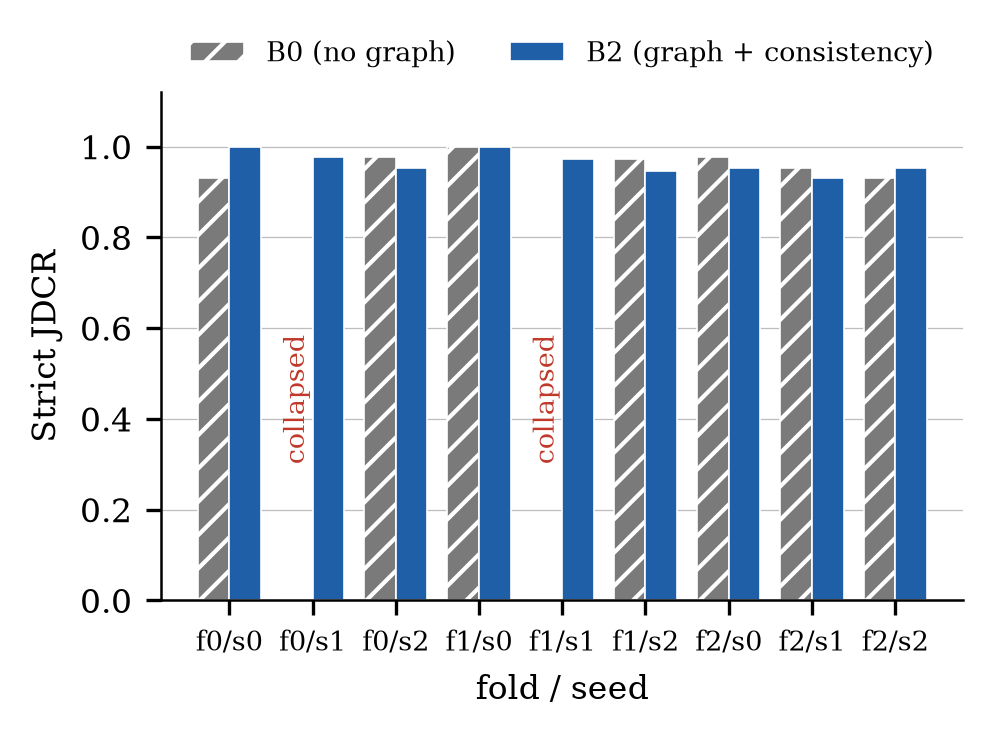
\includegraphics[width=\columnwidth]{figures/fig_jdcr_grid.png}
\caption{Strict JDCR for every fold/seed run. B0's two collapsed runs (empty prediction for every subject) score exactly 0 and produce the mean gap; elsewhere the two models are close.}
\label{fig:jdcr}
\end{figure}

\begin{figure}[t]
\centering
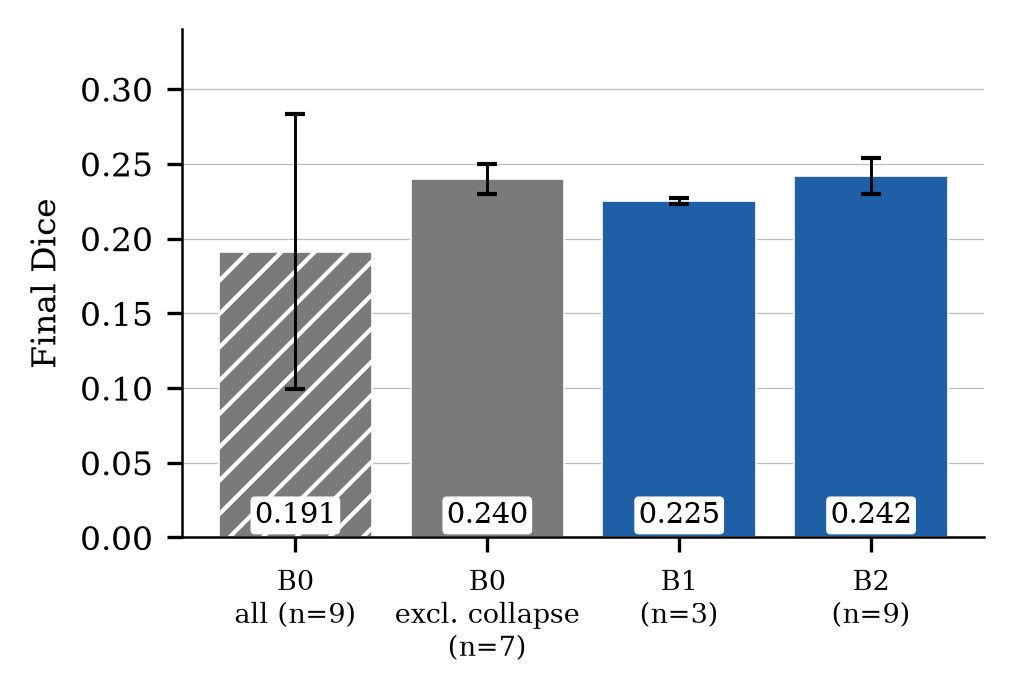
\includegraphics[width=\columnwidth]{figures/fig_dice_summary.png}
\caption{Final Dice, mean $\pm$ SD over runs. B0 is shown with and without its two collapsed runs.}
\label{fig:dice}
\end{figure}

\subsection{Is the graph pathway carrying information?}
Two interventions on B1 (fold 0, 3 seeds) test this directly. \textbf{Random edges:} replacing the 12 anatomical edges with 12 random ones gives Dice $0.2263\pm0.0008$ vs.\ $0.2247\pm0.0024$ for the real anatomy, and JDCR 0.977 vs.\ 0.969. \textbf{Forced-open gate:} initializing $g=1.0$ rather than 0 leaves the gate at $1.00$--$1.03$ throughout training and changes Dice by $-0.0007$ on average. Neither intervention changes accuracy, so the learned pathway, as designed, carries no accuracy-relevant information.

Two further checks agree. A second collateral operationalisation (intact communicating-artery route in the patient's graph) was null against final volume ($n=144$) and admission NIHSS ($n=141$); the communicating arteries are segmented in only 30--48\% of subjects, so ``absent'' is partly a segmentation-sensitivity effect. Against expert TopCoW annotations of 26 of our subjects, our vessel-presence features agree on 91.8\% of 182 comparisons (the anterior communicating artery is weakest at 76.9\%), and disagreement does not predict Dice ($\rho=-0.13$, $p\approx0.5$).

\subsection{Knowledge-grounded failure detection}
Using only inference-time quantities, a prediction is flagged if (a) its lesion mass lies on the side inconsistent with the admission occlusion side, or (b) its predicted volume is under 1\,mL. Thresholds were set from signal distributions, not Dice. (An earlier version also used calibration error, which depends on the true label; we removed it, and the result became stronger.) Over all 1038 (subject, checkpoint) pairs, flagged predictions have median Dice 0.000 against 0.1995 for unflagged ones (Mann--Whitney $p=1.4\times10^{-50}$, AUROC 0.89). The effect holds within B1 and B2 alone, which never collapsed ($p=0.0055$ and $1.5\times10^{-5}$).

Against baselines, severe failure is Dice $<0.05$ (fixed beforehand). On 297 subject-seed predictions from folds 0--1 (Table~\ref{tab:fail}, Fig.~\ref{fig:fail}), the knowledge flag beats ensemble disagreement from B0's 3 seeds. Of 156 severe failures, the flag alone catches 69.2\%, disagreement alone 32.7\%, and together 81.4\%; 18.6\% are missed by both. All 76 failures that only the flag catches are real failures, whereas disagreement's 40 unique catches are only 47.5\% real.

\begin{table}[t]
\centering
\caption{Detecting severe failure (Dice $<0.05$), $n=297$.}
\label{tab:fail}
\footnotesize
\begin{tabular}{lcc}
\toprule
\textbf{Signal} & \textbf{Spearman $\rho$ vs.\ Dice} & \textbf{AUROC} \\
\midrule
Knowledge flag & $-0.754$ & \textbf{0.836} \\
Ensemble disagreement & $-0.214$ & 0.583 \\
Volume coeff.\ of variation & $-0.186$ & 0.575 \\
\bottomrule
\end{tabular}
\end{table}

\begin{figure*}[t]
\centering
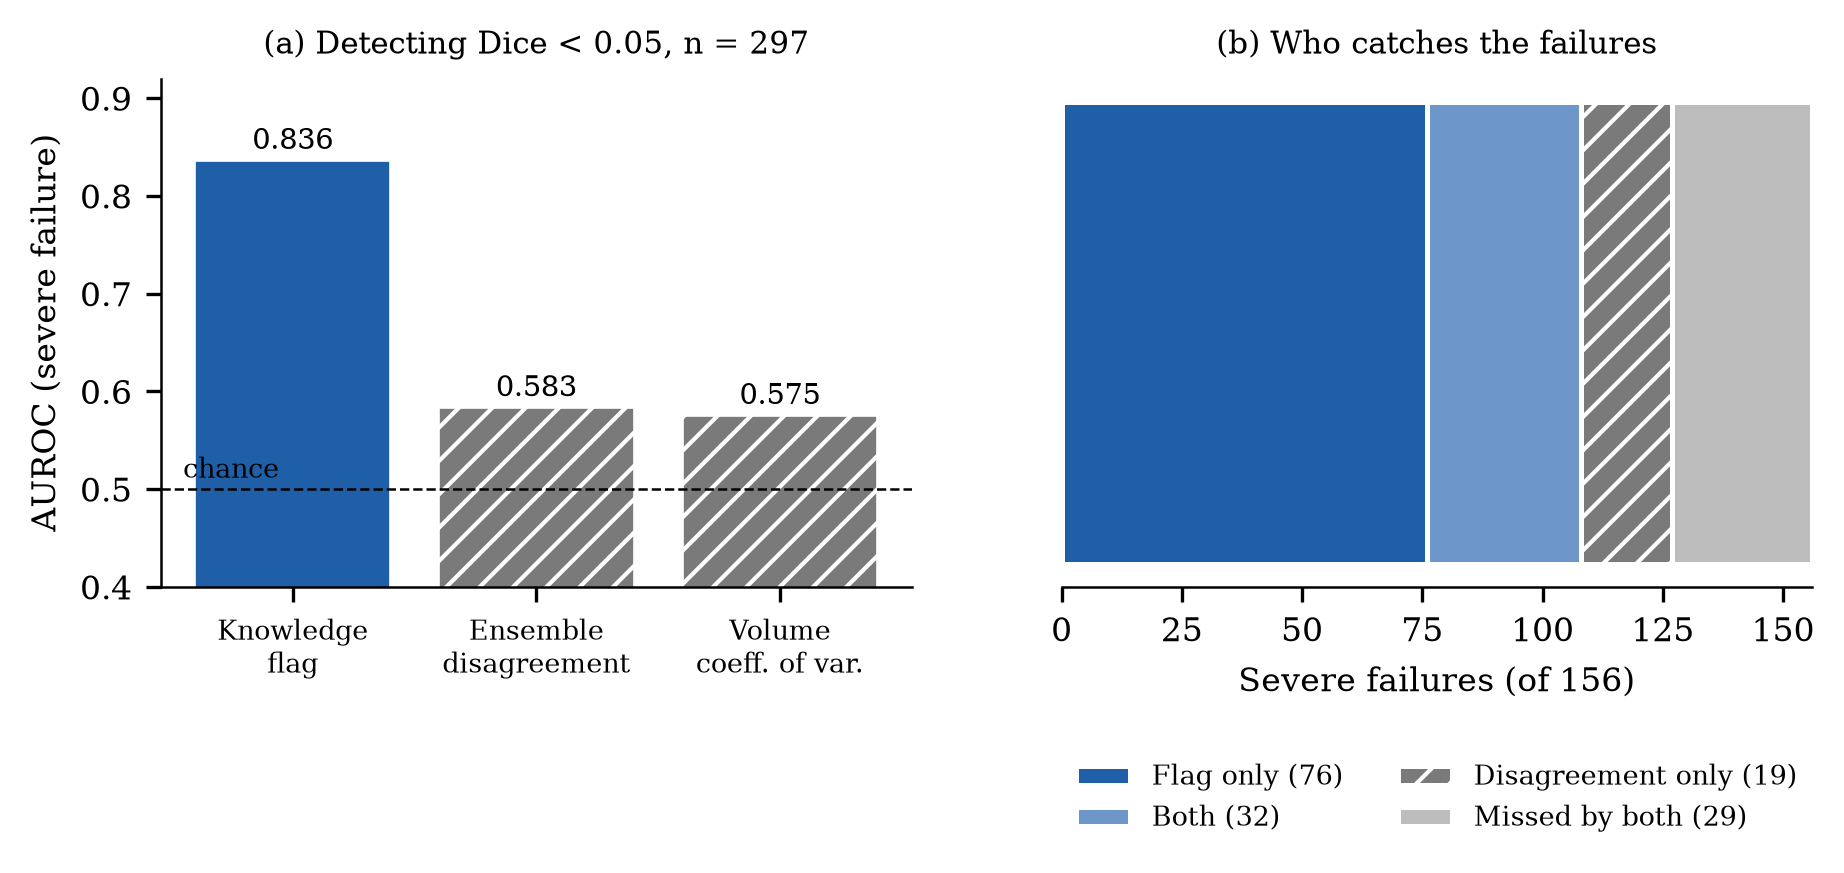
\includegraphics[width=0.85\textwidth]{figures/fig_failure_detection.png}
\caption{(a) AUROC for detecting severe segmentation failure (Dice $<0.05$), $n=297$. (b) Of 156 severe failures, which signal catches them: the knowledge flag only, both, ensemble disagreement only, or neither.}
\label{fig:fail}
\end{figure*}

\textbf{MC-dropout.} On a smaller, single-model, collapse-free subset (fold 0, seed 0, 50 subjects, 6 passes; the architecture has one dropout layer), MC-dropout volume variation scores AUROC 0.819 against 0.652 for the knowledge flag. The subsets differ, so the comparisons are not directly comparable. Together they suggest the knowledge flag dominates on catastrophic, structurally unambiguous failures, while a statistical signal is competitive or better on subtler ones.

\section{Discussion}
\textbf{Validate rules before using them.} Six of seven plausible guideline rules fail in this cohort. Injecting all of them would likely have trained the model against its own data.

\textbf{Where the graph helped.} The learned pathway did not move accuracy under any condition we tried, including interventions meant to give it the best chance. The same graph used as a fixed rule check gave the one result that is large and beats a standard baseline. A knowledge graph's value need not be in what a network learns from it.

\textbf{Mean comparisons can hide outliers.} The pre-registered claim passes on its literal definition, but a paired test shows two extreme runs drive it. We report the pass as registered and do not read it as more than it is.

\section{Limitations}
\begin{itemize}
\item One public dataset with 2 centers; no claim is made about generalization, and the base paper's 7-center results are not reproduced.
\item The cause of B0's two collapses is not determined.
\item The auxiliary heads are unlearnable here at this scale and label quality; this does not say the tasks are unlearnable in general.
\item The MC-dropout comparison covers one model, fold and seed. A matched-scope re-run is not done.
\item The rule results reflect a fully reperfused cohort and may differ in untreated patients.
\item The segmentation target (final infarct) differs from the base paper's admission core/penumbra target.
\end{itemize}

\section{Conclusion}
KG-XAI combines a patient-specific vessel graph, a cohort-validated laterality constraint and a deterministic rule evaluator. Only one of seven guideline rules held in the data. The graph-injected learned pathway did not improve Dice or, under normal training, JDCR; its clear benefits are no observed training collapse and lower calibration error. Used as a non-learned rule check, the same graph detected severe segmentation failure better than ensemble disagreement (AUROC 0.836 vs.\ 0.583), with a competitive MC-dropout baseline on subtler failures. Matched-scope baselines and an external dataset are the next steps.

\section*{Acknowledgment}
We thank the ISLES'24 organizers for the public release and the authors of \cite{luan2026} for the problem framing.

\begin{thebibliography}{00}
\bibitem{luan2026} T. Luan \emph{et al.}, ``Unified multimodal learning for stroke triage: joint detection, scoring, and segmentation of acute ischemic stroke,'' \emph{npj Digital Medicine}, vol. 9, p. 441, 2026.
\bibitem{isles2024} E. O. Riedel \emph{et al.}, ``The ISLES'24 dataset,'' \emph{Radiology: Artificial Intelligence}, vol. 8, no. 3, 2026, doi: 10.1148/ryai.250603.
\bibitem{myronenko2018} A. Myronenko, ``3D MRI brain tumor segmentation using autoencoder regularization,'' in \emph{Int. MICCAI Brainlesion Workshop}, 2018, pp. 311--320.
\bibitem{velickovic2018} P. Veli\v{c}kovi\'{c} \emph{et al.}, ``Graph attention networks,'' in \emph{Proc. ICLR}, 2018.
\bibitem{topcow2023} K. Yang \emph{et al.}, ``TopCoW: Benchmarking topology-aware anatomical segmentation of the circle of Willis (CoW) for CTA and MRA,'' arXiv:2312.17670, 2023.
\bibitem{alastruey2007} J. Alastruey \emph{et al.}, ``Modelling the circle of Willis to assess the effects of anatomical variations and occlusions on cerebral blood flow,'' \emph{J. Biomechanics}, vol. 40, no. 8, pp. 1794--1805, 2007.
\bibitem{dawn2018} R. G. Nogueira \emph{et al.}, ``Thrombectomy 6 to 24 hours after stroke with a mismatch between deficit and infarct,'' \emph{N. Engl. J. Med.}, vol. 378, no. 1, pp. 11--21, 2018.
\bibitem{defuse3_2018} G. W. Albers \emph{et al.}, ``Thrombectomy for stroke at 6 to 16 hours with selection by perfusion imaging,'' \emph{N. Engl. J. Med.}, vol. 378, no. 8, pp. 708--718, 2018.
\bibitem{ahaasa2026} S. Prabhakaran \emph{et al.}, ``2026 Guideline for the management of patients with acute ischemic stroke,'' \emph{Stroke}, vol. 57, no. 8, pp. e316--e436, 2026.
\bibitem{olivot2014} J. M. Olivot \emph{et al.}, ``Hypoperfusion intensity ratio predicts infarct progression and functional outcome in the DEFUSE 2 cohort,'' \emph{Stroke}, vol. 45, no. 4, pp. 1018--1023, 2014.
\bibitem{lakshminarayanan2017} B. Lakshminarayanan, A. Pritzel, and C. Blundell, ``Simple and scalable predictive uncertainty estimation using deep ensembles,'' in \emph{Proc. NeurIPS}, 2017.
\bibitem{gal2016dropout} Y. Gal and Z. Ghahramani, ``Dropout as a Bayesian approximation: representing model uncertainty in deep learning,'' in \emph{Proc. ICML}, 2016.
\end{thebibliography}

\end{document}
